\begin{enumerate}
%%Ejercicio 1
\item
\begin{enumerate}
\item Si el universo es finito podemos tomar $U_I=\mathbb{N}_{[4,9,16,25]}\ $ y la funci�n  $f_1(x,y)= \sqrt{x}.\sqrt{y}\ $o si el universo es infinito simplemente podemos tomar los Reales de 1 a 10 $U_I=\mathbb{R}_{(1..10]}\ $ y la misma funci�n me sirve para los dos casos.
\item TODO
\item Podemos tomar $U_I = \mathbb{N}_{[0,..,10]}\ $ y la funci�n $f_1(x,y) = x.y\ $ donde $y\ $ ser�a la constanste $c_1 = 0\ $. Si quisieramos un universo infinito simplemente podr�amos tomar los Naturales con el cero.
\end{enumerate}\smallskip
%%Ejercicio 2
\item
\begin{enumerate}
\item $\forall x \exists y (f(x,y)=c)\ $ Este enunciado no es universalmente v�lido porque pues para los Naturales o los Enteros no vale.
\item $\forall x \exists y (f(x,y)=c)\ $ Solo vale para los complejos.
\end{enumerate}\smallskip
%%Ejercicio 3
\item
\begin{enumerate}
\item $\alpha: \forall x \exists y (f(x,y)=c\ $ donde $c_1 = 0$ 
\item $\beta:  $
\item $\gamma: $
\end{enumerate}\smallskip
%%Ejercicio 4
\item
\begin{enumerate}
\item Sea $I_1: U_I = \mathbb{C},\  f_1(x) = x^2\ $  \newline
Esta interpretaci�n funciona para $\alpha\ $ pu�s la inversa de la funci�n $f_1(x)\ $ no se indefine en los complejos, asi que siempre podr� obtener un $f(y) = x\ $. Sin embargo si vemos $\beta\ $ notaremos que el enunciado no se cumple para esta funci�n ya que $f_1(x) = f_1(-x)\ $ y  $x \not= -x$
\item 
\end{enumerate}
%%Ejercicio 5
\item
\begin{enumerate}
\item $\exists x \forall y  (x\leq y)$
\item Vamos a usar el s�mbolo $\bullet$ para indicar que $x \bullet y \longleftrightarrow (\neg(x\leq y) \land \neg(y\leq x))$\newline
Tambi�n usaremos el s�mbolo $\not =$ para indicar que $x \not = y \longleftrightarrow \neg((x \leq y) \land (y\leq x))$\newline
La idea es que en el primer gr�fico hay 4 n�meros (1,2,3,4) entre los cuales no hay una relaci�n de orden, es decir, ninguno es menor o igual al otro y adem�s que para cualquier otro n�mero distinto a ellos, dicho n�mero es mayor.\newline
$\exists x,y,w,z,t ((x\bullet y)\land (x\bullet w) \land (x\bullet z) \land (y\bullet w) \land (y\bullet z) \land (w\bullet z)  \land (t \not = x) \land (t\not = y) \land (t\not = w) \land (t\not = z))\rightarrow$ \newline
$\forall t( (x\leq t)\lor (y\leq t) \lor (w\leq t) \lor (z\leq t))$
\end{enumerate}\smallskip
%%Ejercicio 6
\item Se grafican a continuaci�n los dos ejemplos, el primero cumple mientras que el segundo no :  \newline

\begin{tikzpicture}[inner sep=0mm]
\tikzstyle{color0}=[circle,fill=white]
\node at (1,2) (nodo1)[color0] {$\bullet_1$};
\node at (0,1) (nodo3)[color0] {$\bullet_2$};
\node at (2,1) (nodo2)[color0] {$\bullet_3$};
\node at (1,0) (nodo4)[color0] {$\bullet_4$};
\draw [->] (nodo1) to [bend left =20](nodo2);
\draw [->] (nodo1) to [bend right = 20](nodo3);
\draw [->] (nodo2) to [bend left = 20] (nodo4);
\draw [->] (nodo3) to [bend right = 20] (nodo4);
%%Reutilc� el c�digo anterior y renombre todos los nodos con el prefijo 2nodo :P
\node at (7,2) (2nodo1)[color0] {$\bullet_1$};
\node at (6,2) (2nodo3)[color0] {$\bullet_2$};
\node at (8,2) (2nodo2)[color0] {$\bullet_3$};
\node at (7,0) (2nodo4)[color0] {$\bullet_4$};
\draw [->] (2nodo1) to (2nodo4);
\draw [->] (2nodo2) to [bend left = 20] (2nodo4);
\draw [->] (2nodo3) to [bend right = 20] (2nodo4);
\end{tikzpicture}\smallskip
%%Ejercicio 7
\item
\begin{enumerate}
\item
\item
\item
\item
\end{enumerate}\newpage
%%Ejercicio 8
\item Para probar que las f�rmulas son equivalentes debemos probar $(\alpha \rightarrow \phi)\ $ y $ (\phi \rightarrow \alpha)\ $, esto lo hacemos negando la primera implicaci�n y demostrando que su �rbol de refutaci�n se cierra, hacemos lo mismo con la implicaci�n para el otro lado y si el �rbol tambi�n se cierra, esto indicar�a que las implicaciones son tautolog�a. En otras palabras las f�rmulas son equivalentes.\newline
Probemos primero que: $\neg(\forall x \exists y (P(x,y) \rightarrow P(y,x)) \rightarrow \forall x \exists y(P(x,y) \rightarrow \exists z P(z,x)))$
\begin{center}
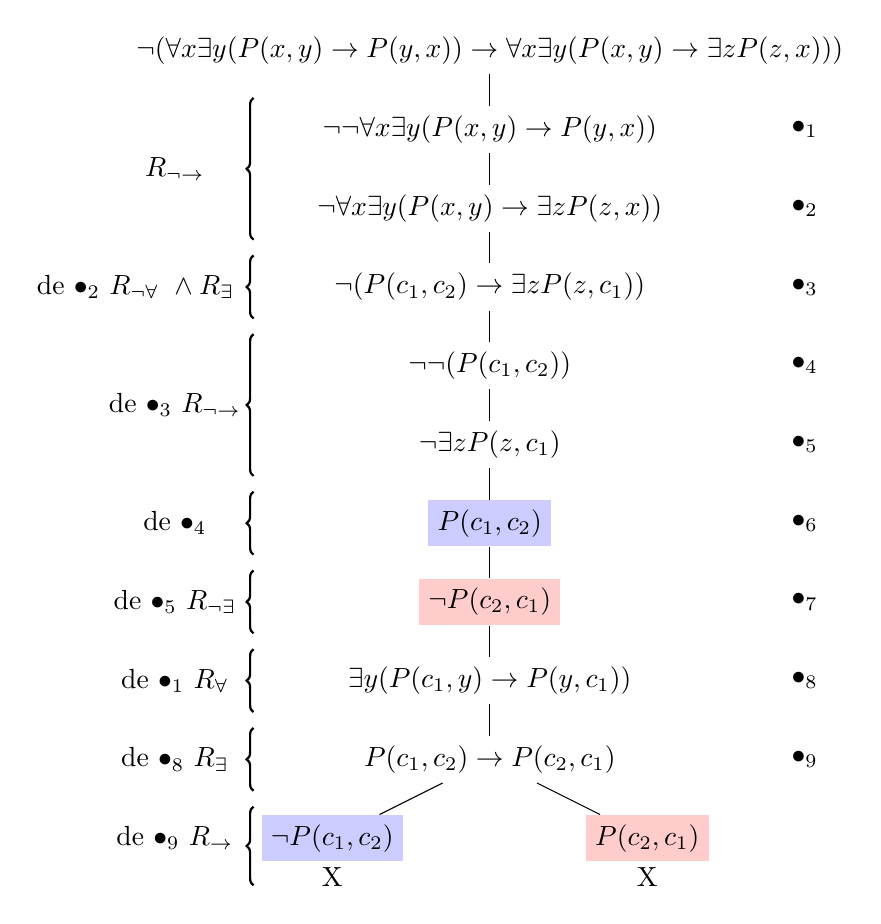
\begin{tikzpicture}
\node at (10,10) (formula1) {$\neg(\forall x \exists y (P(x,y) \rightarrow P(y,x)) \rightarrow \forall x \exists y(P(x,y) \rightarrow \exists z P(z,x)))$};
\node at (10,9) (formula2) {$\neg \neg \forall x \exists y (P(x,y) \rightarrow P(y,x))$};
\node at (14,9) (de1) {$\bullet_1$};
\node at (10,8) (formula3) {$\neg \forall x \exists y(P(x,y) \rightarrow \exists z P(z,x))$};
\node at (14,8) (de2) {$\bullet_2$};
\node at (10,7) (formula4) {$\neg(P(c_1,c_2) \rightarrow \exists z P(z,c_1))$};
\node at (14,7) (de3) {$\bullet_3$};
\node at (10,6) (formula5) {$\neg\neg(P(c_1,c_2))$};
\node at (14,6) (de4) {$\bullet_4$};
\node at (10,5) (formula6) {$\neg \exists z P(z,c_1)$};
\node at (14,5) (de5) {$\bullet_5$};
\node at (10,4) (formula7) [rectangle,fill=blue!20] {$P(c_1,c_2)$};
\node at (14,4) (de6) {$\bullet_6$};
\node at (10,3) (formula8) [rectangle,fill=red!20] {$\neg P(c_2,c_1)$};
\node at (14,3) (de7) {$\bullet_7$};
\node at (10,2) (formula9) {$\exists y (P(c_1,y) \rightarrow P(y,c_1))$};
\node at (14,2) (de8) {$\bullet_8$};
\node at (10,1) (formula10) {$P(c_1,c_2) \rightarrow P(c_2,c_1)$};
\node at (14,1) (de9) {$\bullet_9$};
\node at (8,0) (formula11a) [rectangle,fill=blue!20]{$\neg P(c_1,c_2)$};
\node at (12,0) (formula11b) [rectangle,fill=red!20] {$P(c_2,c_1)$};
\node at (8,-0.5) (x1) {X};
\node at (12,-0.5) (x2) {X};

\draw [-] (formula1) to (formula2);
\draw [-] (formula2) to (formula3);
\draw [-] (formula3) to (formula4);
\draw [-] (formula4) to (formula5);
\draw [-] (formula5) to (formula6);
\draw [-] (formula6) to (formula7);
\draw [-] (formula7) to (formula8);
\draw [-] (formula8) to (formula9);
\draw [-] (formula9) to (formula10);
\draw [-] (formula10) to (formula11a);
\draw [-] (formula10) to (formula11b);

\draw [decorate,decoration=brace,thick]  (7,7.6) -- (7,9.4);
\draw [decorate,decoration=brace,thick] (7,6.6) -- (7,7.4);
\draw [decorate,decoration=brace,thick] (7,4.6) -- (7,6.4);
\draw [decorate,decoration=brace,thick] (7,3.6) -- (7,4.4);
\draw [decorate,decoration=brace,thick] (7,2.6) -- (7,3.4);
\draw [decorate,decoration=brace,thick] (7,1.6) -- (7,2.4);
\draw [decorate,decoration=brace,thick] (7,0.6) -- (7,1.4);
\draw [decorate,decoration=brace,thick] (7,-0.6) -- (7,0.4);

\node at (6,8.5) (nodo1) {$R_{\neg \rightarrow}$};
\node at (5.5,7) (nodo2) {de $\bullet_2\ R_{\neg \forall}\ \land R_{\exists}$};
\node at (6,5.5) (nodo3) {de $\bullet_3\ R_{\neg \rightarrow}$};
\node at (6,4) (nodo4) {de $\bullet_4$};
\node at (6,3) (nodo5) {de $\bullet_5 \ R_{\neg \exists}$};
\node at (6,2) (nodo6) {de $\bullet_1 \ R_{\forall}$};
\node at (6,1) (nodo7) {de $\bullet_8 \ R_{\exists}$};
\node at (6,0) (nodo7) {de $\bullet_9 \ R_{\rightarrow}$};

\end{tikzpicture}\smallskip
\end{center}
En el punto 3 tengo un $\neg \forall\ $ y un $\exists \ $ de modo que los reemplazo por dos constantes $c_1, c_2\ $ distintas.\newline
En el punto 5 tengo un $\neg \exists\ $ y como lo puedo reemplazar por cualquier cosa, uso $c_2$. \newline
En el punto 8 tengo un $\exists \ $ y como ya lo hab�a reemplazado por $c_2\ $ uso la misma constante en este caso.\newline
\newpage %Salto de pagina

Ahora analizamos la siguiente implicaci�n: $\neg(\forall x \exists y(P(x,y) \rightarrow \exists z P(z,x)) \rightarrow \forall x \exists y (P(x,y) \rightarrow P(y,x)))$
\begin{center}
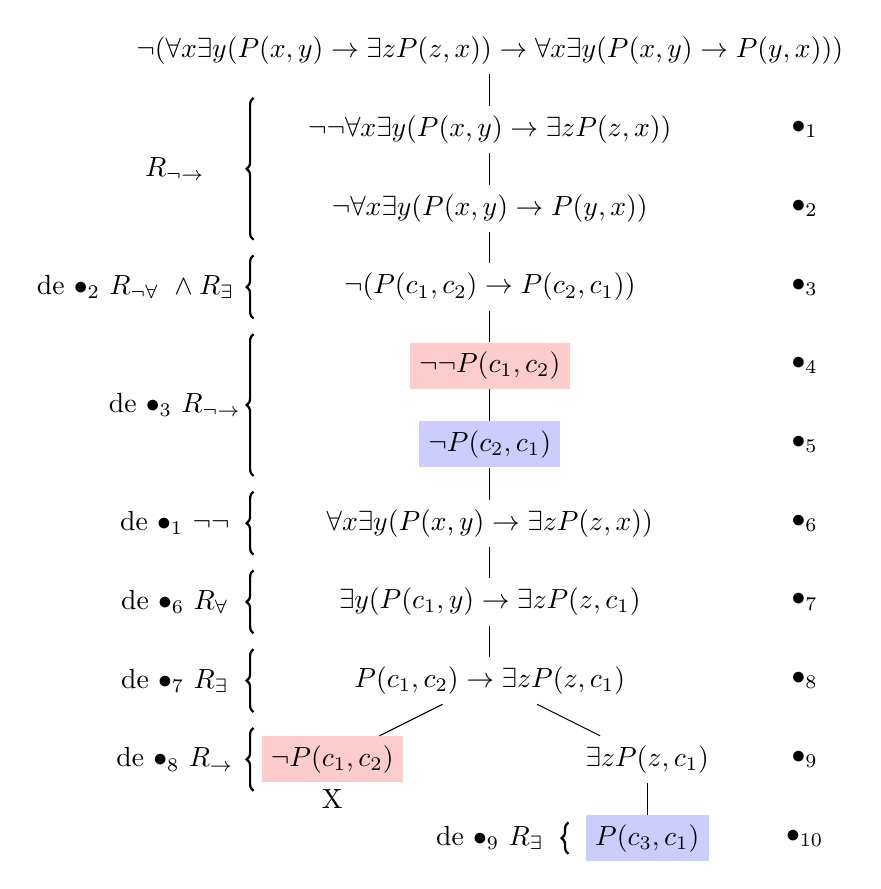
\begin{tikzpicture}
\node at (10,10) (formula1) {$\neg(\forall x \exists y(P(x,y) \rightarrow \exists z P(z,x)) \rightarrow \forall x \exists y (P(x,y) \rightarrow P(y,x)))$};
\node at (10,9) (formula2) {$\neg \neg \forall x \exists y(P(x,y) \rightarrow \exists z P(z,x))$};
\node at (14,9) (de1) {$\bullet_1$};
\node at (10,8) (formula3) {$\neg \forall x \exists y (P(x,y) \rightarrow P(y,x))$};
\node at (14,8) (de2) {$\bullet_2$};
\node at (10,7) (formula4) {$\neg(P(c_1,c_2) \rightarrow P(c_2,c_1))$};
\node at (14,7) (de3) {$\bullet_3$};
\node at (10,6) (formula5) [rectangle,fill=red!20] {$\neg \neg P(c_1,c_2)$};
\node at (14,6) (de4) {$\bullet_4$};
\node at (10,5) (formula6) [rectangle,fill=blue!20] {$\neg P(c_2,c_1)$};
\node at (14,5) (de5) {$\bullet_5$};
\node at (10,4) (formula7) {$\forall x \exists y(P(x,y) \rightarrow \exists z P(z,x))$};
\node at (14,4) (de6) {$\bullet_6$};
\node at (10,3) (formula8) {$\exists y(P(c_1,y) \rightarrow \exists z P(z,c_1)$};
\node at (14,3) (de7) {$\bullet_7$};
\node at (10,2) (formula9) {$P(c_1,c_2) \rightarrow \exists z P(z,c_1)$};
\node at (14,2) (de8) {$\bullet_8$};
\node at (8,1) (formula10a) [rectangle,fill=red!20] {$\neg P(c_1,c_2)$};
\node at (12,1) (formula10b) {$\exists z P(z,c_1)$};
\node at (14,1) (de9) {$\bullet_9$};
\node at (12,0) (formula11b) [rectangle,fill=blue!20]{$P(c_3,c_1)$};
\node at (14,0) (de10b) {$\bullet_{10}$};
\node at (8,0.5) (formula11a) {X};

\draw [-] (formula1) to (formula2);
\draw [-] (formula2) to (formula3);
\draw [-] (formula3) to (formula4);
\draw [-] (formula4) to (formula5);
\draw [-] (formula5) to (formula6);
\draw [-] (formula6) to (formula7);
\draw [-] (formula7) to (formula8);
\draw [-] (formula8) to (formula9);
\draw [-] (formula9) to (formula10a);
\draw [-] (formula9) to (formula10b);
\draw [-] (formula10b) to (formula11b);

\draw [decorate,decoration=brace,thick]  (7,7.6) -- (7,9.4);
\draw [decorate,decoration=brace,thick] (7,6.6) -- (7,7.4);
\draw [decorate,decoration=brace,thick] (7,4.6) -- (7,6.4);
\draw [decorate,decoration=brace,thick] (7,3.6) -- (7,4.4);
\draw [decorate,decoration=brace,thick] (7,2.6) -- (7,3.4);
\draw [decorate,decoration=brace,thick] (7,1.6) -- (7,2.4);
\draw [decorate,decoration=brace,thick] (7,0.6) -- (7,1.4);
\draw [decorate,decoration=brace,thick] (11,-0.2) -- (11,0.2);

\node at (6,8.5) (nodo1) {$R_{\neg \rightarrow}$};
\node at (5.5,7) (nodo2) {de $\bullet_2\ R_{\neg \forall}\ \land R_{\exists}$};
\node at (6,5.5) (nodo3) {de $\bullet_3\ R_{\neg \rightarrow}$};
\node at (6,4) (nodo4) {de $\bullet_1\ \neg \neg$};
\node at (6,3) (nodo5) {de $\bullet_6 \ R_{\forall}$};
\node at (6,2) (nodo6) {de $\bullet_7 \ R_{\exists}$};
\node at (6,1) (nodo7) {de $\bullet_8 \ R_{\rightarrow}$};
\node at (10,0) (nodo8) {de $\bullet_9 \ R_{\exists}$};
\end{tikzpicture}\smallskip
\end{center}
Observemos que en $\bullet_{10}\ $ la rama solo se cierra si $c_3 = c_2\ $ de otro modo las f�rmulas no ser�an equivalentes.
\newpage
%%Ejercicio 9
\item
\begin{enumerate}
\item Para probar que la f�rmula es universalmente v�lida debo demostrar que su negaci�n es una contradicci�n, esto lo probamos mediante el m�todo de �rboles de refutaci�n, basta ver que es cerrado.\newline
Negamos la f�rmula : $\neg (\exists y P(y) \rightarrow \forall x \exists y P(y))$\newline\medskip
\begin{center}
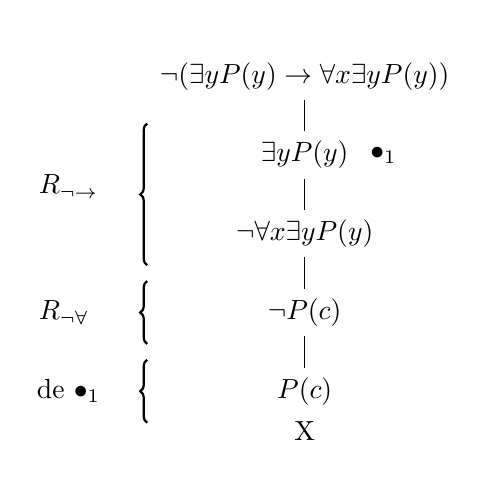
\begin{tikzpicture}
\node at (0,0.5) (dummy) {};%%Para dejar un rengl�n
\node at (0,0) (formula1){$\neg (\exists y P(y) \rightarrow \forall x \exists y P(y))$};
\node at (0,-1) (formula2) {$ \exists y P(y)$}; \node at (1,-1) (1) {$\bullet_1$};
\node at (0,-2) (formula3) {$\neg \forall x \exists y P(y)$};
\node at (0,-3) (formula4) {$\neg P(c)$};
\node at (0,-4) (formula5) {$P(c)$};
\node at (0,-4.5) (fin) {X};

\draw [-] (formula1) to (formula2);
\draw [-] (formula2) to (formula3);
\draw [-] (formula3) to (formula4);
\draw [-] (formula4) to (formula5);

\draw [decorate,decoration=brace,thick]  (-2,-2.4) -- (-2,-0.6);
\draw [decorate,decoration=brace,thick] (-2,-3.4) -- (-2,-2.6);
\draw [decorate,decoration=brace,thick] (-2,-4.4) -- (-2,-3.6);
\node at (-3,-1.4) (nodo1) {$R_{\neg \rightarrow}$};
\node at (-3,-3) (nodo2) {$R_{\neg \forall}\ $};
\node at (-3,-4) (nodo3) {de $\bullet_1$};
\end{tikzpicture}\smallskip
\end{center}
\item Procedemos de la misma manera que en la parte a)\newline
Negamos la f�rmula: $\neg(\exists y P(y) \rightarrow \exists y \exists x P(y))$ \newline
\begin{center}
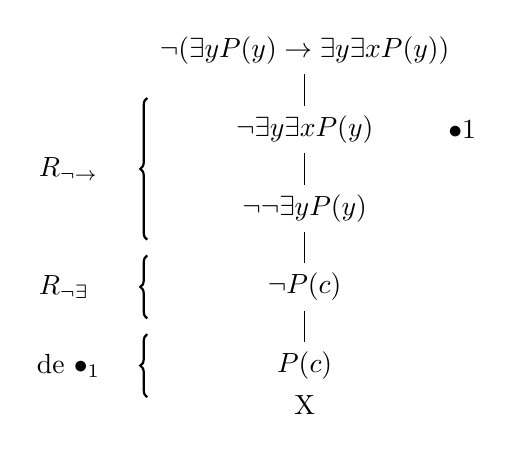
\begin{tikzpicture}
\node at (10,10) (formula1) {$\neg(\exists y P(y) \rightarrow \exists y \exists x P(y))$};
\node at (10,9) (formula2) {$ \neg \exists y \exists x P(y)$};
\node at (12,9) (de1) {$\bullet{1}$};
\node at (10,8) (formula3) {$\neg \neg \exists y P(y) $};
\node at (10,7) (formula4) {$\neg P(c)$};
\node at (10,6) (formula5) {$P(c)$};
\node at (10,5.5) (x) {X};

\draw [-] (formula1) to (formula2);
\draw [-] (formula2) to (formula3);
\draw [-] (formula3) to (formula4);
\draw [-] (formula4) to (formula5);

\draw [decorate,decoration=brace,thick]  (8,7.6) -- (8,9.4);
\draw [decorate,decoration=brace,thick] (8,6.6) -- (8,7.4);
\draw [decorate,decoration=brace,thick] (8,5.6) -- (8,6.4);

\node at (7,8.5) (nodo1) {$R_{\neg \rightarrow}$};
\node at (7,7) (nodo2) {$R_{\neg \exists}\ $};
\node at (7,6) (nodo3) {de $\bullet_1$};
\end{tikzpicture}
\end{center}\smallskip

\item Misma idea, negamos la f�rmula: $\neg(\forall x P(x) \rightarrow P(t))$\newline
\begin{center}
\begin{tikzpicture}
\node at (10,10) (formula1) {$\neg(\forall x P(x) \rightarrow P(t))$};
\node at (10,9) (formula2) {$\neg P(t)$};
\node at (12,9) (de1) {$\bullet{1}$};
\node at (10,8) (formula3) {$\neg\neg(\forall x P(x)$};
\node at (10,7) (formula 4) {$P(t)$};
\node at (10,6) (formula 5) {$\neg P(t)$};
\node at (10,5.5) (x) {X};

\draw [-] (formula1) to (formula2);
\draw [-] (formula2) to (formula3);
\draw [-] (formula3) to (formula4);
\draw [-] (formula4) to (formula5);

\draw [decorate,decoration=brace,thick]  (8,7.6) -- (8,9.4);
\draw [decorate,decoration=brace,thick] (8,6.6) -- (8,7.4);
\draw [decorate,decoration=brace,thick] (8,5.6) -- (8,6.4);

\node at (7,8.5) (nodo1) {$R_{\neg \rightarrow}$};
\node at (7,7) (nodo2) {$R_{\forall}\ $};
\node at (7,6) (nodo3) {de $\bullet_1$};
\end{tikzpicture}
\end{center}
\end{enumerate}\smallskip
\newpage
%%Ejercicio 10
\item
\begin{enumerate}
\item
Debemos introducir reglas de expansi�n para el $\leftrightarrow $ esto es lo mismo que, dadas dos funciones $\alpha\ $ y $\phi$, $(\alpha \rightarrow  \phi) \land (\phi \rightarrow \alpha)$.

De Modo que:

$R_\leftrightarrow = (\alpha \rightarrow  \phi) \land (\phi \rightarrow \alpha) \ $y

$R_{\neg \leftrightarrow} = \neg(\alpha \rightarrow  \phi) \lor \neg(\phi \rightarrow \alpha) \ $
\begin{center}
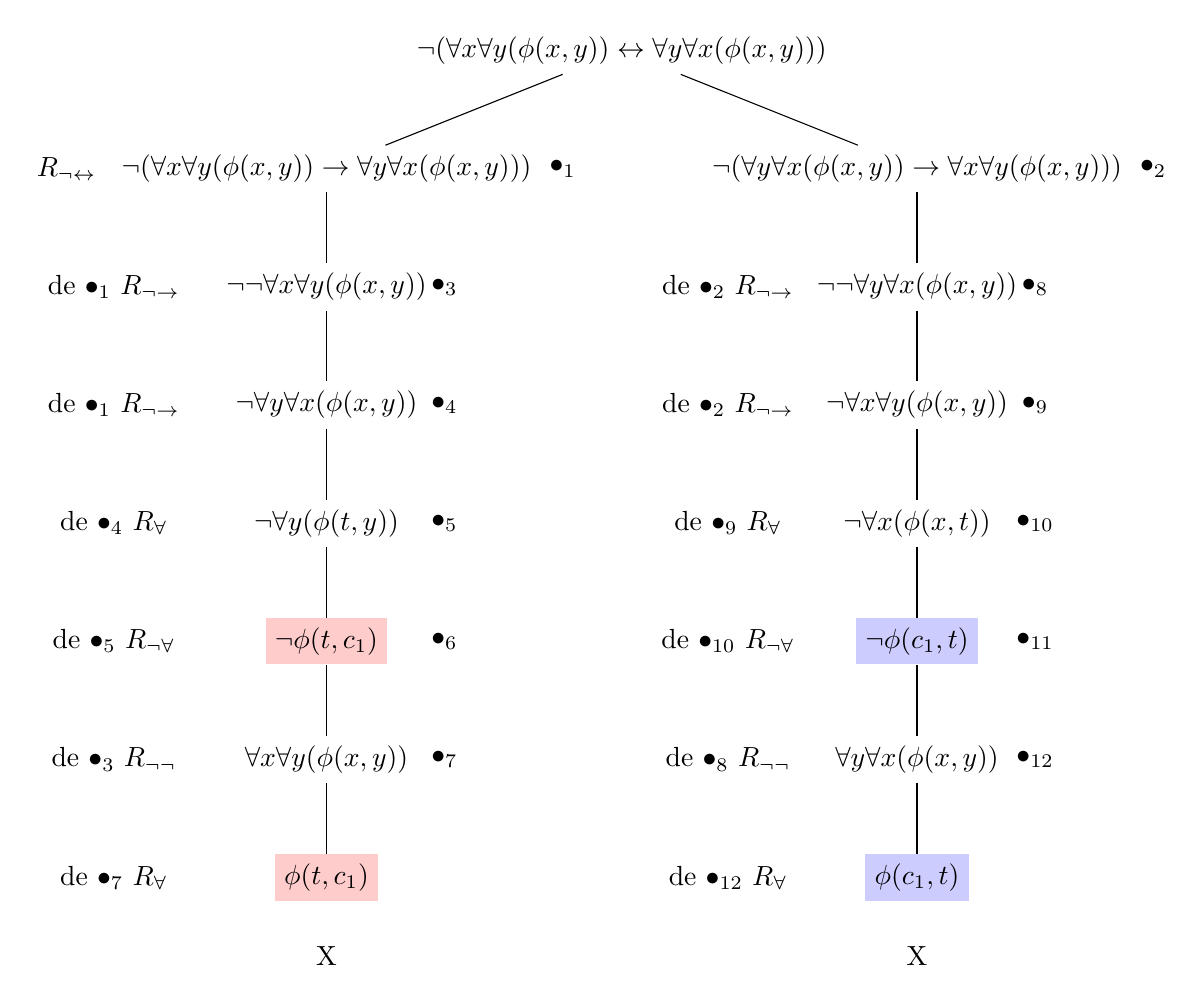
\begin{tikzpicture}
[level 1/.append style={sibling distance=7.5cm}]
\node (raiz) {$ \neg(\forall x \forall y (\phi (x,y)) \leftrightarrow  \forall y \forall x (\phi (x,y)))$} % root
child { node (hijo1) {$\neg (\forall x \forall y (\phi (x,y)) \rightarrow  \forall y \forall x (\phi (x,y)))$}
	child {node (nieto1){$\neg \neg\forall x \forall y (\phi (x,y))$}
		child {node (bisnieto1){$ \neg \forall y \forall x (\phi (x,y))$}
			child {node (tnieto1){$\neg \forall y(\phi(t,y))$}
				child {node (tnieto12) [rectangle,fill=red!20] {$\neg \phi(t,c_1)$}
					child {node (tnieto13) {$\forall x \forall y (\phi (x,y))$}
						child {node (tnieto14) [rectangle,fill=red!20] {$\phi(t,c_1)$}}}}}}}}						
child { node (hijo2) {$\neg (\forall y \forall x (\phi (x,y)) \rightarrow  \forall x \forall y (\phi (x,y))) $}
	child {node (nieto2){$\neg \neg\forall y \forall x (\phi (x,y))$}
		child {node (bisnieto2){$ \neg \forall x \forall y (\phi (x,y))$}
			child {node (tnieto2){$\neg \forall x(\phi(x,t))$}
				child {node (tnieto22) [rectangle,fill=blue!20]{$\neg \phi(c_1,t)$}
					child {node (tnieto23) {$\forall y \forall x (\phi (x,y))$}
						child {node (tnieto24) [rectangle,fill=blue!20] {$\phi(c_1,t)$}}}}}}}};
\node [below of = tnieto14] {X};						
\node [below of = tnieto24] {X};
\node (nodo1) [node distance=3cm,right of = hijo1] {$\bullet_1$} ;
\node (nodo2) [node distance=3cm, right of = hijo2] {$\bullet_2$};
\node (nodo3) [node distance=1.5cm, right of = nieto1] {$\bullet_3$};
\node (nodo4) [node distance=1.5cm, right of = bisnieto1] {$\bullet_4$};
\node (nodo5) [node distance=1.5cm, right of = tnieto1] {$\bullet_5$};
\node (nodo6) [node distance=1.5cm, right of = tnieto12] {$\bullet_6$};
\node (nodo7) [node distance=1.5cm, right of = tnieto13] {$\bullet_7$};
\node (nodo3) [node distance=1.5cm, right of = nieto2] {$\bullet_8$};
\node (nodo4) [node distance=1.5cm, right of = bisnieto2] {$\bullet_9$};
\node (nodo5) [node distance=1.5cm, right of = tnieto2] {$\bullet_{10}$};
\node (nodo6) [node distance=1.5cm, right of = tnieto22] {$\bullet_{11}$};
\node (nodo7) [node distance=1.5cm, right of = tnieto23] {$\bullet_{12}$};

\node (nodo8) [node distance=3.3cm, left of =  hijo1] { $R_{\neg \leftrightarrow }$};
\node (nodo8) [node distance=2.7cm, left of =  nieto1] { de $\bullet_{1}\ R_{\neg \rightarrow}$};
\node (nodo9) [node distance=2.7cm, left of =  bisnieto1] { de $\bullet_{1}\ R_{\neg \rightarrow}$};
\node (nodo10) [node distance=2.7cm, left of = tnieto1] { de $\bullet_{4}\ R_{\forall}$};
\node (nodo11) [node distance=2.7cm, left of = tnieto12] { de $\bullet_{5}\ R_{\neg \forall}$};
\node (nodo12) [node distance=2.7cm, left of = tnieto13] { de $\bullet_{3}\ R_{\neg \neg}$};
\node (nodo13) [node distance=2.7cm, left of = tnieto14] { de $\bullet_{7}\ R_{\forall}$};

\node (nodo14) [node distance=2.4cm, left of =  nieto2] { de $\bullet_{2}\ R_{\neg \rightarrow}$};
\node (nodo15) [node distance=2.4cm, left of =  bisnieto2] { de $\bullet_{2}\ R_{\neg \rightarrow}$};
\node (nodo16) [node distance=2.4cm, left of = tnieto2] { de $\bullet_{9}\ R_{\forall}$};
\node (nodo17) [node distance=2.4cm, left of = tnieto22] { de $\bullet_{10}\ R_{\neg \forall}$};
\node (nodo18) [node distance=2.4cm, left of = tnieto23] { de $\bullet_{8}\ R_{\neg \neg}$};
\node (nodo19) [node distance=2.4cm, left of = tnieto24] { de $\bullet_{12}\ R_{\forall}$};
\end{tikzpicture}
\end{center}
\end{enumerate}
\end{enumerate}